\section{Numerische Auswertung}

\begin{frame}{Numerische Auswertung}
    \begin{itemize}
        \item<1-> Für die numerischen Verfahren wurden die Python Bibliotheken \textbf{numpy} und \textbf{scipy} verwendet.
        \item<2-> Die Implementationen der numerischen Verfahren beschränken sich auf die Funktionen
        \texttt{scipy.integrate.RK45} für das Runge-Kutta-Verfahren und \texttt{scipy.integrate.BDF} für das BDF-Verfahren.
        \item<3-> Das neuronale Netz wurde mit der Bibliothek \textbf{tensorflow} implementiert.
    \end{itemize}
\end{frame}

\begin{frame}{Numerische Auswertung: Fehlermaße}
    \begin{itemize}
        \item<1-> Zum Vergleich der Verfahren werden verschiedene Fehlermaße betrachtet.
        \item<2-> Es werden die \textbf{Trajektorien} verglichen.
        \begin{itemize}
            \item<1-> Eine Trajektorie ist das Bild $T(x_0)=\{x(t,x_0):t\in I_{\text{max}} \}$ der Lösung des
            Anfangswertproblems mit dem maximalen Existenzintervall $I_{\text{max}}$.
        \end{itemize}
        \item<3-> Die globalen Fehler $\left\lVert x(t_i) - u_i \right\rVert_2$ der numerischen Verfahren werden mit den
        globalen Fehler der neuronalen Netze $\left\lVert x(t_i) - \hat{x}(t_i) \right\rVert_2$ für $t_i=t_0+ih$ verglichen.
        \begin{itemize}
            \item<1-> Für diesen Vergleich muss die exakte Lösung $x$ gegeben sein.
        \end{itemize}
        \item<4-> Falls keine exakte Lösung vorliegt, wird eine Referenzlösung zum Vergleich der Trajektorien genutzt.
    \end{itemize}
\end{frame}

\begin{frame}{Numerische Auswertung: Fehlermaße}
    \begin{itemize}
        \item<1-> Es werden die $(x_1,t)$-Graphen verglichen, dabei ist $x_1$ die erste Orskomponente des AWP´s
        \item<2-> Es werden die Kostenfunktion und, wenn möglich der Fehler des neuronalen Netzes für steigende Epochen
        angegeben.
    \end{itemize}
\end{frame}

\subsection{Rebound-Pendel}

\begin{frame}{Rebound-Pendel}
    \begin{itemize}
        \item<1-> Das Rebound-Pendel ist ein Anfangswertproblem erster Ordnung der Form
        \begin{align}
            \theta^{\prime} &= \varphi, \nonumber \\
            \varphi^{\prime} &= - \frac{g}{l} \sin(\theta) + H(-\theta)
            \text{ReLU}(-\frac{kl}{m}\theta - c \varphi), \label{rebound-pendulum}\\
            \theta(0) &= 1, \quad \varphi(0)=0.2 \nonumber
        \end{align}
        mit $\text{ReLU}(x)= \max(x, 0)$,
        \begin{align*}
            H(x) =
            \begin{cases}
                0, &x<0 \\
                1, &x \geq 0
            \end{cases},
        \end{align*}
        $g$ die Erdbeschleunigung, $l$ die Länge des Pendels, $m$ die Masse des Pendels, $k$ die Federkonstante und $c$ der
        Dämpfungskoeffizient.
    \end{itemize}
\end{frame}

\begin{frame}{Rebound-Pendel: Abbildung}
    TODO:CITE
    \begin{figure}
        \centering
        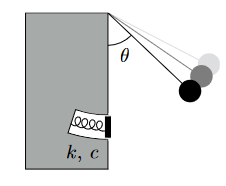
\includegraphics{images/rebound_pendulum_diagram}
        \caption{Diagramm eines Rebound Pendels\cite[6]{flamantSolvingDifferentialEquations2020}}
        \label{fig:rebound_pendulum_diagram}
    \end{figure}
\end{frame}

\subsection{Steife Differentialgleichung}

\begin{frame}{Steife Differentialgleichung}
    \begin{itemize}
        \item<1-> Es wird das Anfangswertproblem \eqref{stiff} betrachtet.
        \item<2-> Für die Parameter gilt $c_1=3$, $c_2=4$, $\lambda_1=-100$ und $\lambda_2=-1$.
        \item<3-> Für die relative und globale Toleranz gilt $rtol=10^{-2}$, $atol=10^{-7}$.
    \end{itemize}
\end{frame}

\subsection{Harmonischer Oszillator}

\begin{frame}{Harmonischer Oszillator}
    \begin{itemize}
        \item<1-> Der harmonische Oszillator ist ein Anfangswerproblem erster Ordnung der Form
        \begin{align*}
            &x^{\prime}=v, \qquad v^{\prime}=-\frac{k}{m}x, \\
            &x(0)=0, \quad v(0)=0.
        \end{align*}
        \item<2-> Für die Parameter gilt $m=1$ und $k=1$ für das Runge-Kutta-Verfahren.
        \item<3-> Für die relative und globale Toleranz gilt $rtol=10^{-10}$, $atol=10^{-14}$.
    \end{itemize}
\end{frame}